%%%%%%%%%%%%%%%%%%%%%%%%%%%%%%%%%%%%%%%%%%%%%%%%%%%%%%%%%%%%%%%%%
% Qualificacao de Doutorado / Dept Fisica, CFM, UFSC            %
% Eduardo@UFSC - 2015                                           %
%%%%%%%%%%%%%%%%%%%%%%%%%%%%%%%%%%%%%%%%%%%%%%%%%%%%%%%%%%%%%%%%%


%:::::::::::::::::::::::::::::::::::::::::::::::::::::::::::::::%
%                                                               %
%                          Capítulo 4                           %
%                                                               %
%:::::::::::::::::::::::::::::::::::::::::::::::::::::::::::::::%

%***************************************************************%
%                                                               %
%                      Conversão tauV - Gas                     %
%                                                               %
%***************************************************************%

\chapter{Coeficiente de extinção como indicador de Gás}
\label{sec:gas}
% Referências:
% - Brinchman
% - Guiderdoni & Rocca
% - procurar mais conversões dust to gas ou dust to stars
% - Referências para cada indicador
\section{Indicadores de gás}
\label{sec:synvsneb:proxies}
% Figuras:
% - ?? retiradas alguns papers para diferentes indicadores ??
\section{Lei de Schimidt-Kennict}
\label{sec:synvsneb:proxies}
% Figuras:
% - sample SK
% - our pseudo - SK
Na figura \ref{fig:pSK_sample} podemos ver a influência dos cortes em $\tau_V$ e $x_Y$ conforme
discutido em \ref{sec:synvsneb:amostra}.

\begin{figure}
	\centering
	%\resizebox{0.99\textwidth}{!}{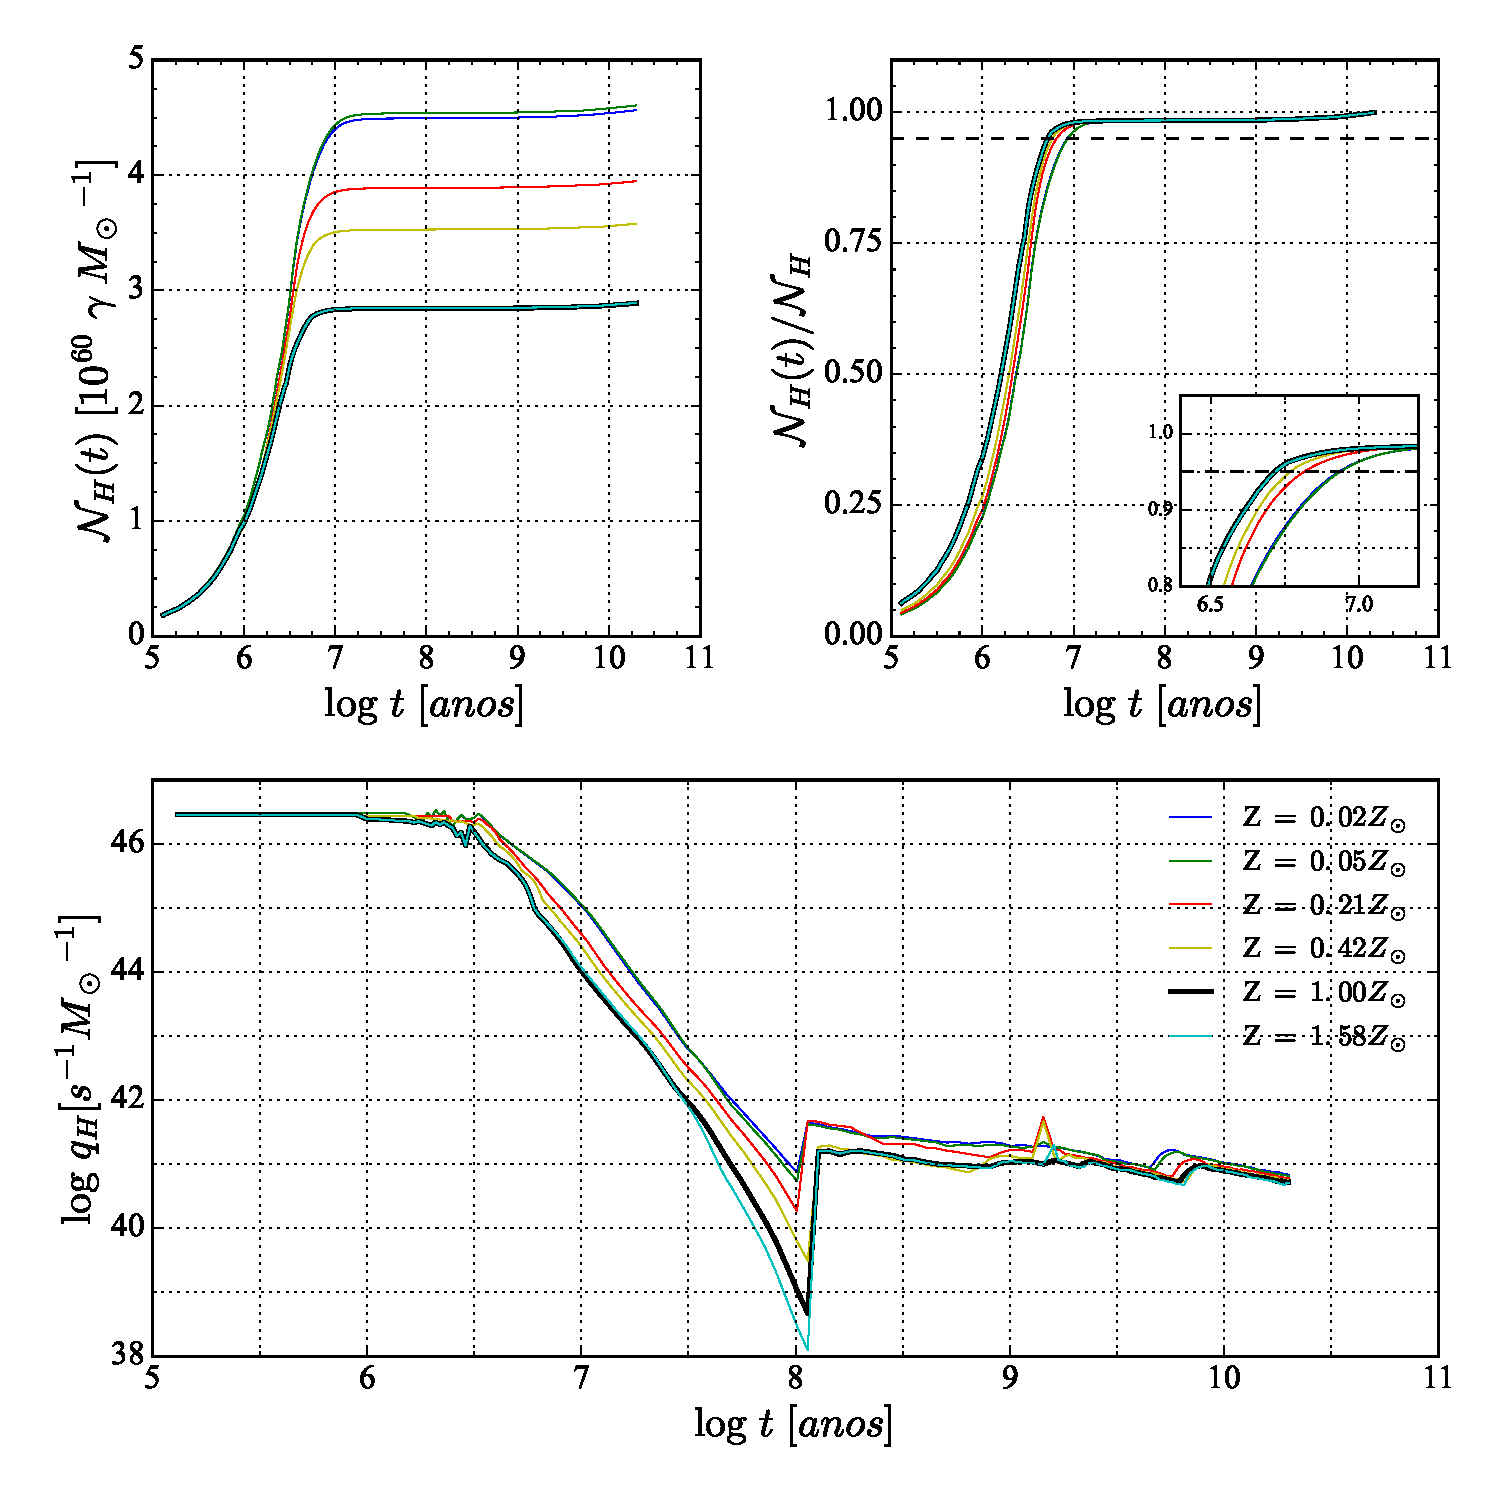
\includegraphics{Nh_logt_metBase_Padova2000_salp.pdf}}
	\includegraphics[scale=1]{figuras/pSKsample.pdf}
	\caption[Efeitos de configuração de mínimo de população jovem e de mínimo coeficiente de extinção.]
	{xxx nononnnnonononononon xxx}
	\label{fig:pSK_sample}
\end{figure}


\section{De poeira para gás}
\label{sec:synvsneb:proxies}
% Figuras:
% - perfis radiais de SigmaGas e de fgas
% - real SK

% End of this chapter
